\section{Agile roles}
\label{sec:agile_roles}
If the system should be implemented at different work environments the role system should be more flexible. 
It is not given that all workplaces can make use of the three predefined roles. 
In fact it is not given at all. 
Therefore a more flexible role system would be more efficient and make the system more agile. 
As it is now each controller has a predefined role which is allowed to access the controllers functionality. 
This method is not very agile and it is impossible for the users to change which roles can access what. 
This can be improved by introducing a double layered role system.  
This work by making a role for each controller or even the controllers action methods. 
Then adding a high level role set which can access the low level roles. 
This allow for agile changing the privileges for an entire group of users. 
E.g. if the user of the system wants to allow clients to see statistics this can easily be changed with this improvement. An example of this alternative role system can be seen on figure \ref{fig:improved_role_system}.

\paragraph{Pros} are that the system allows more specific configuration. 
\paragraph{Cons} are not existing.
\paragraph{We did not implement this feature because} it is not one of the main important features of the project.

\begin{figure}
\begin{center}
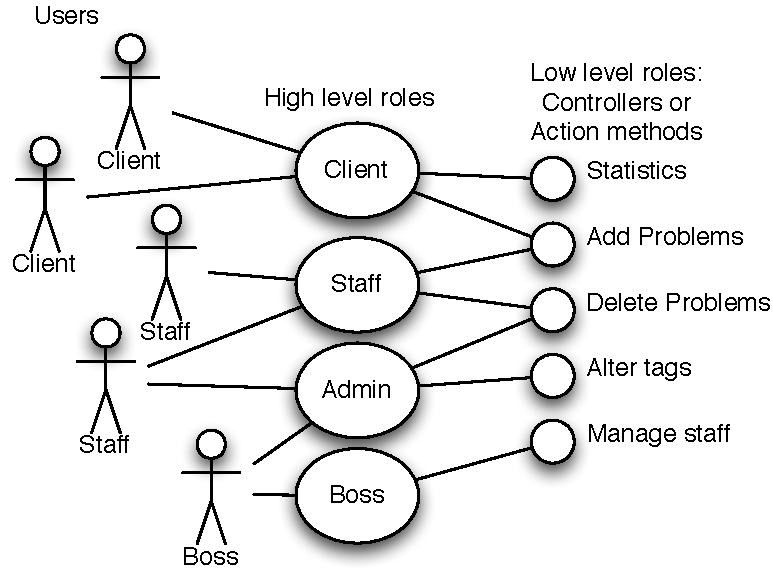
\includegraphics[scale=1]{input/epilogue/improvements/improved_role_system.pdf}
\caption{Example of how the roles can be structured with an improved role system}
\label{fig:improved_role_system}
\end{center}
\end{figure}
